\documentclass{article}


\setlength{\textwidth}{164mm} \setlength{\textheight}{23.0cm}
\setlength{\headheight}{0cm} \setlength{\topmargin}{-0.1cm}
\setlength{\oddsidemargin}{0cm} \setlength{\evensidemargin}{0cm}
\setlength{\parskip}{1mm} \setlength{\unitlength}{1mm}
\def\baselinestretch{1.1}

%\usepackage[active]{srcltx}

\usepackage{amsmath}
\usepackage{amsthm}
\usepackage{txfonts}
\usepackage{fancybox}
\usepackage{color}
\usepackage{booktabs}
\usepackage{ulem}
\usepackage[dvips]{graphicx}
\usepackage{caption2}
\usepackage{amssymb}
\usepackage{amsbsy}
\usepackage{longtable}
\usepackage{dsfont}
%
%\usepackage{hhline}


\newtheorem{algorithm}{Algorithm}

\title{Graphical Models}
\author{Jinlong Wu \& Tiejun Li}
\date{Nov 2008}

\begin{document}
\maketitle
%\sloppy
\section{Introduction}
Jordan \cite{Jordan} presentes a very concise introduction to \textit{Graphical Models (GMs)}:

\begin{minipage}[c]{0.94\textwidth}
\quad\ \textsf{Graphical models are a marriage between probability theory and graph theory. They provide
a natural tool for dealing with two problems that occur throughout applied mathematics and
engineering --- uncertainty and complexity --- and in particular they are playing an increasingly
important role in the design and analysis of machine learning algorithms. Fundamental to the
idea of a graphical model is the notion of modularity --- a complex system is built by combining
simpler parts. Probability theory provides the glue whereby the parts are combined, ensuring
that the system as a whole is consistent, and providing ways to interface models to data. The
graph theoretic side of graphical models provides both an intuitively appealing interface by which
humans can model highly-interacting sets of variables as well as a data structure that lends itself
naturally to the design of efficient general-purpose algorithms.}

\quad\ \textsf{Many of the classical multivariate probabilistic systems studied in fields such as statistics,
systems engineering, information theory, pattern recognition and statistical mechanics are special
cases of the general graphical model formalism --- examples include mixture models, factor analysis,
hidden Markov models, Kalman filters and Ising models. The graphical model framework provides
a way to view all of these systems as instances of a common underlying formalism. This view has
many advantages --- in particular, specialized techniques that have been developed in one field can
be transferred between research communities and exploited more widely. Moreover, the graphical
model formalism provides a natural framework for the design of new systems.
}
\end{minipage}\\

GMs are usually divided into two types --- \textit{undirected} and \textit{directed}.
Undirected GMs are also called \textit{Markov Networks} or \textit{Markov Random Fields (MRFs)},
and directed GMs are also known as \textit{Bayesian Networks (BNs)}, \textit{belief networks},
\textit{generative models} or \textit{causal models}.

\subsection{Directed GMs (Bayesian Networks) \cite{Murphy}}
In Bayesian Networks (BNs) each vertex represents a random variable, and an arc
from vertex $X$ to vertex $Y$ (we also said that $X$ is one of the parents of $Y$)
means $X$ is one of the reasons why $Y$ happens, i.e., $X$ causes $Y$.
Hence BNs are acyclic.
BNs assume that a variable is independent of its ancestors given its parents,
and use the notation ``$\Perp$'' to show the conditional independence.

A simple example is shown in Figure \ref{wetgrass}.
We can write $R\!\!\Perp\!\!S|C$ and $W\!\!\Perp\!\!C|S,R$ according to the conditional independence.
\begin{figure}[h]
\centering
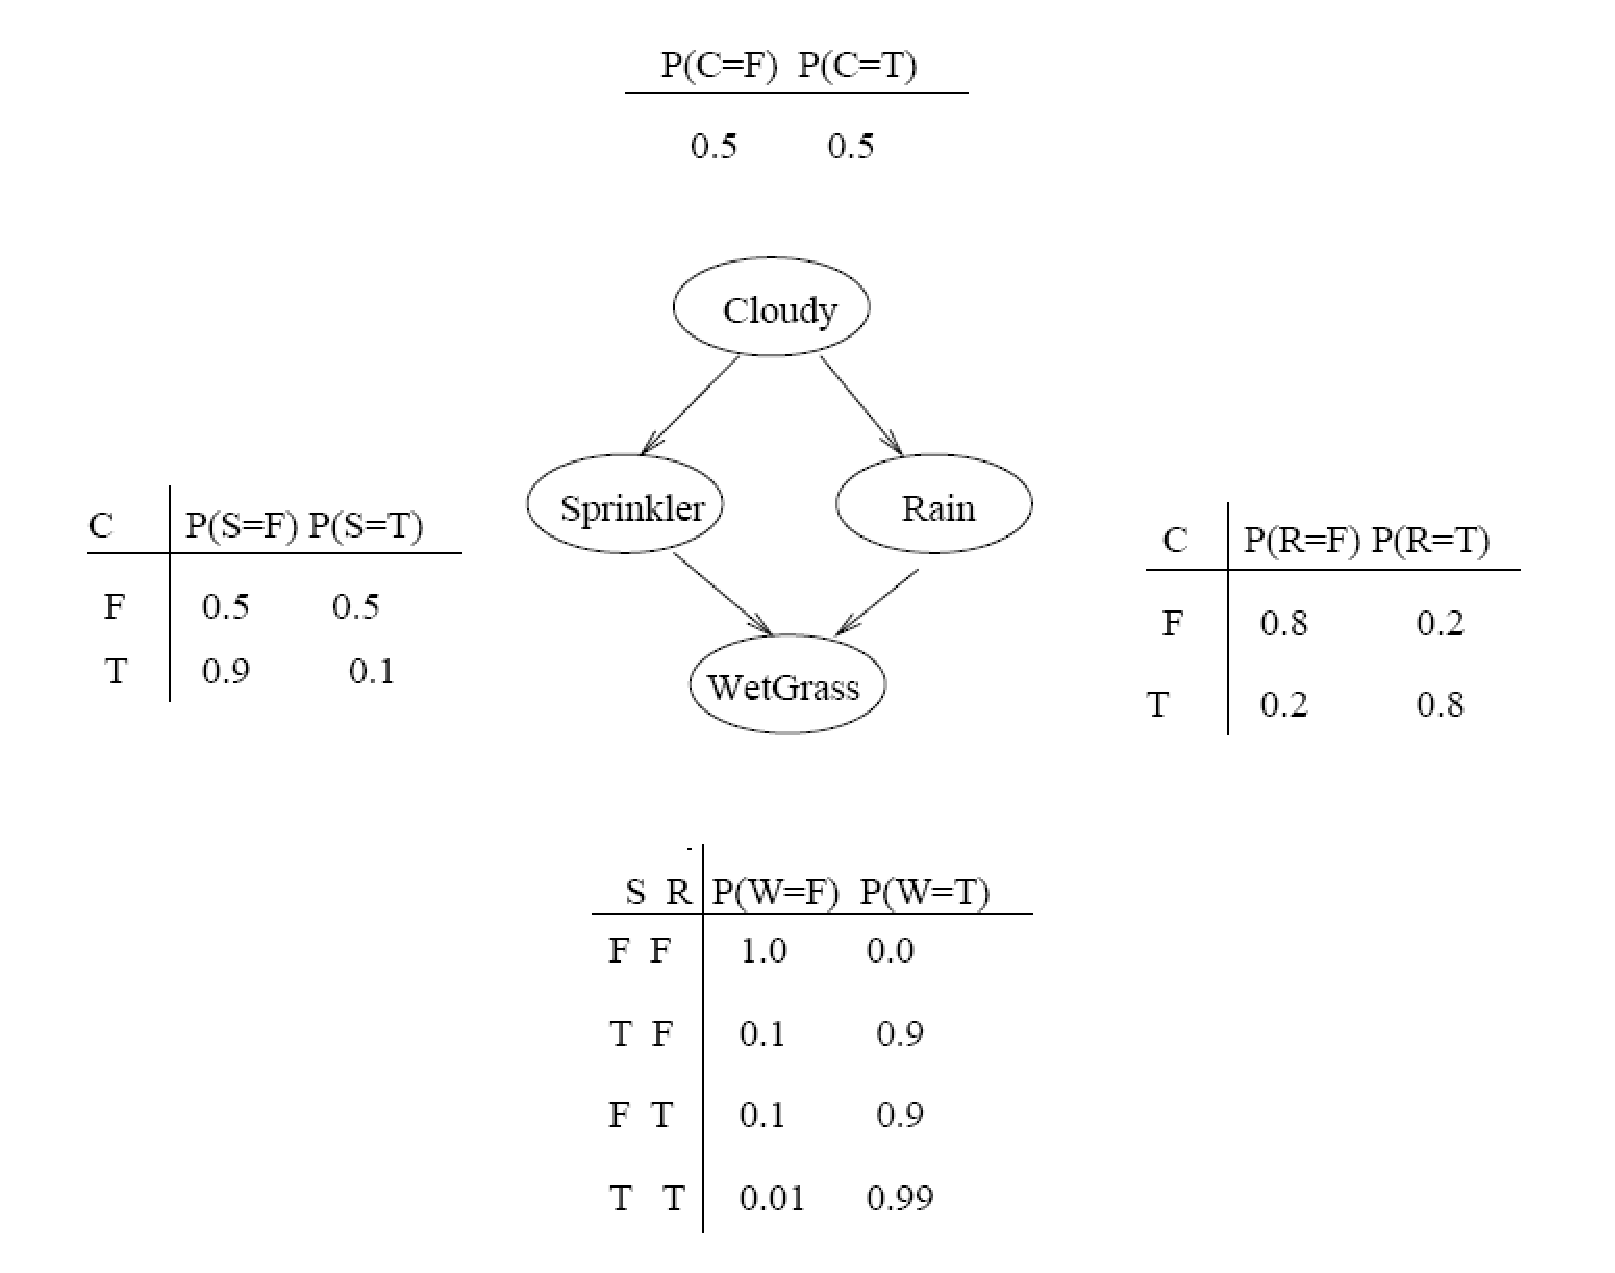
\includegraphics[trim=0 10 0 0,width=0.95\textwidth]{wetgrass2.eps}
\caption{A simple Bayesian network from \cite{Russell} and the related CPTs.}\label{wetgrass}
\end{figure}
The tables around the BNs are the \textit{conditional probability tables (CPTs)} of the
corresponding variables.
According to the above assumption, the joint probability of all the variables is
$$
P(C, S, R, W) = P(C)  P(S|C)  P(R|C)  P(W|S,R) \quad .
$$

\subsection{Undirected Graphical Models (Markov Random Fields) \cite{Murphy}}
The joint distribution of a Markov Random Field (MRF) is defined by
\begin{equation}
P(X) = \frac{1}{\Xi} \prod_{C\in\mathcal{C}} \psi_C(X_C)
\end{equation}
where $\mathcal{C}$ is the set of maximal cliques in the graph, $\psi_C(X_C)$ is a potential
function (a positive, but otherwise arbitrary, real-valued function) on the clique $X_C$,
and $\Xi$ is the normalization factor
\begin{equation}
\Xi = \sum_X \prod_{C\in\mathcal{C}} \psi_C(X_C) \quad .
\end{equation}

Consider the example in Figure \ref{mrf}.  In this case, the joint distribution is
\begin{equation}
P(X,Y) \propto \Psi(X_1,X_2)\Psi(X_1,X_3)\Psi(X_2,X_4)\Psi(X_3,X_4)\prod_{i=1}^4\Psi(X_i,Y_i) \quad .
\end{equation}
\begin{figure}[h]
\centering
\includegraphics[trim=100 160 210 120,width=0.95\textwidth]{mrf.eps}
\caption{A Markov Random Field for low level vision. $X_i$ is the hidden state of the world at grid position
$i$, and $Y_i$ is the corresponding observed state.}\label{mrf}
\end{figure}

In low-level vision problems, the $X_i$ are usually hidden, and each $X_i$ node has its own
``private'' observation node $Y_i$, as in Figure \ref{mrf}.
The potential $\Psi(X_i,Y_i)=P(Y_i|X_i)$ encodes the local likelihood;
this is often a conditional Gaussian, where $Y_i$ is the image intensity of pixel $i$, and
$X_i$ is the underlying (discrete) scene ``label''.

\section{Inference and Learning}
The main goal of inference is to estimate the values of hidden nodes, given the values of the observed nodes.
It is usually based on Bayes' rule.
Learning might refer to the structure (topology) of the model, or the parameters, or both \cite{Murphy}.

Many algorithms for exact inference have been developed, such as \textit{dynamic programming},
\textit{forwards-backwards} for HMMs and so forth.
However, these exact algorithms are time-consuming exponentially in the size of the largest
cluster (also called the \textit{induced width} of the graph) if all hidden nodes are discrete.
Approximate inference is often much more popular for GMs.
Some approximate inference methods are listed as follows.
See more details in \cite{Murphy} and its references.
\begin{itemize}
  \item Sampling (Monte Carlo) methods, such as \textit{Importance Sampling},
  \textit{Markov Chain Monte Carlo (MCMC)}.
  \item Variational methods, such as the \textit{mean-field approximation}.
  \item Loopy belief propagation.
\end{itemize}

It is beyond the scope of this chapter to discuss how to learn the structure of models.
In the following we only discuss some methods to learn the parameters.
Some common methods to learn the parameters is to find the parameters to maximize or
minimize some objective function, such as
\begin{itemize}
\item to find the maximum likelihood estimates (MLEs) of the parameters;
\item to find the maximum a posterori (MAP) estimates of the parameters;
\item to find the parameters to minimize a type of error functions
(usually MSE or MAE for regression, and cross-entropy for classification).
\end{itemize}
After determining the objective function, we can use \textit{Gradient Descent (Ascent)},
\textit{Expectation Maximization}, \textit{Variational Methods} or
other methods to achieve good estimates of the parameters.


\section{Variational Methods for ML/MAP Learning}
Consider a generative model with hidden variables $Z$ and observed variables $X$.
The observed data set $x=\{x_1,\ldots, x_N\}$ is assumed to be sampled
from the model independently.
Hence the log-likelihood as a function of the parameters $\Theta$ is
\begin{equation}
\mathcal{L}(\Theta)=\log P(x|\Theta) = \sum^N_{n=1} \log P(x_n|\Theta)
= \sum^N_{n=1} \log\int P(x_n,z_n|\Theta) dz_n \quad .
\end{equation}
Maximum Likelihood (ML) tries to find the parameters $\Theta_{ML}$ to maximize
the likelihood, or equivalently, to maximize the log-likelihood $\mathcal{L}(\Theta)$.
That is,
\begin{equation}
\Theta_{ML} = {\arg\ \max}_{\Theta} \mathcal{L}(\Theta) \quad .
\end{equation}

In Bayesian networks without hidden variables, $\mathcal{L}(\Theta)$ usually can
decompose into local terms on each data point $x_n$, and so all parameters in $\mathcal{L}(\Theta)$
are decoupled, which makes the maximum problem easy.
Unfortunately, if there exist some hidden variables, all parameters typically
couple together, which makes the problem hard to solve.

The maximum problem usually can be simplified by introducing an auxiliary distribution $q_z(z)$ over
the hidden variables (called \textit{$q$-distribution}).
In fact, for each data point $x_n$ we use a distinct distribution
$q_{z_n}(z_n)$ over the hidden variables, which gives rise to a lower bound on $\mathcal{L}(\Theta)$
\begin{eqnarray}
\mathcal{L}(\Theta) &=& \sum^N_{n=1} \log\int P(x_n,z_n|\Theta) dz_n \\
&=& \sum^N_{n=1} \log\int q_{z_n}(z_n) \frac{P(x_n,z_n|\Theta)}{q_{z_n}(z_n)}dz_n \\
&\geq& \sum^N_{n=1} \int q_{z_n}(z_n) \log\frac{P(x_n,z_n|\Theta)}{q_{z_n}(z_n)}dz_n \label{lf}\\
&=& \sum^N_{n=1}\Bigl[ \int q_{z_n}(z_n)\log P(x_n,z_n|\Theta)dz_n-
\int q_{z_n}(z_n)\log q_{z_n}(z_n)dz_n \Bigr]\label{freeenergy}\\
&\equiv& \mathcal{F}(q_{z_1}(z_1),\ldots,q_{z_n}(z_n);\Theta) \quad .
\end{eqnarray}
$\mathcal{F}(q_{z_1}(z_1),\ldots,q_{z_n}(z_n);\Theta)$ is called the \textit{free energy}.

Since $\mathcal{F}$ is always a lower bound on $\mathcal{L}$, and maximizing $\mathcal{L}$
is difficult, we maximize $\mathcal{F}$ over $q_z(z)$ and $\Theta$ instead of $\mathcal{L}$.

\subsection{Variational Methods for Unconstrained Distribution over Hidden Variables --- EM}
The Expectation Maximization (EM) algorithm alternates between E-Step and
M-Step.  The E-Step updates the posterior distribution over hidden variables given the current parameter values,
and the M-Step updates the parameters given the posterior distribution.
In this subsection, we will derive the EM algorithm by maximizing
$\mathcal{F}(q_{z_1}(z_1),\ldots,q_{z_n}(z_n);\Theta)$
when $q$-distribution can be any distribution.

To maximize $\mathcal{F}$, we update the $q$-distribution and the parameters $\Theta$
iteratively.  The update steps can be achieved by differentiating $\mathcal{F}$
with respect $q_{z_n}(z_n)$ and $\Theta$, and setting the derivatives to zero respectively.
The details are shown in the following.

When updating $q_{z_n}(z_n)$, we should notice the normalization constraints
\begin{equation}
\int q_{z_n}(z_n) dz_n = 1 \ , \quad\forall n = 1,\ldots,N
\end{equation}
since $q_{z_n}(z_n)$ are density functions.  The constraints can be incorporated into
the objective function by Lagrange multipliers method perfectly to achieve a new objective function
\begin{equation}
\hat{\mathcal{F}}(q_z(z);\Theta) = \mathcal{F}(q_z(z);\Theta)
+ \sum^N_{n=1} \lambda_n \Bigl[ \int q_{z_n}(z_n) dz_n - 1 \Bigr ] \quad .
\end{equation}
Setting the derivative to zero,
\begin{eqnarray}
\frac{\partial}{\partial q_{z_n}(z_n)} \hat{\mathcal{F}}(q_z(z);\Theta^{(t)})
&=& \log P(x_n,z_n|\Theta^{(t)}) - \log q_{z_n}(z_n) - 1 + \lambda_n \\
&=& 0 \quad ,
\end{eqnarray}
we get
\begin{equation}\label{qe-step}
q_{z_n}^{(t+1)}(z_n) = P(z_n|x_n, \Theta^{(t)}) \ , \quad\forall n = 1,\ldots,N
\end{equation}
where the superscript $(t)$ shows it is the value after the $t$-th iteration.
The previous equation makes the inequality in (\ref{lf}) become an equality
\footnote{
We can rewrite the free energy $\mathcal{F}$
\begin{eqnarray}
\mathcal{F}(q_{z_1}(z_1),\ldots,q_{z_n}(z_n);\Theta)
&=& \sum^N_{n=1} \int q_{z_n}(z_n) \log\frac{P(x_n,z_n|\Theta)}{q_{z_n}(z_n)}dz_n \nonumber\\
&=& \sum^N_{n=1} \int q_{z_n}(z_n) \log P(x_n|\Theta)dz_n +
\sum^N_{n=1} \int q_{z_n}(z_n) \log\frac{P(z_n|x_n,\Theta)}{q_{z_n}(z_n)}dz_n \nonumber\\
&=& \sum^N_{n=1} \log P(x_n|\Theta) -
\sum^N_{n=1} \int q_{z_n}(z_n) \log\frac{q_{z_n}(z_n)}{P(z_n|x_n,\Theta)}dz_n \nonumber\\
&\equiv& \sum^N_{n=1} \log P(x_n|\Theta) - \sum^N_{n=1} \text{KL}[q_{z_n}(z_n)\parallel P(z_n|x_n,\Theta)] \nonumber\quad,
\end{eqnarray}
where $\text{KL}[q_{z_n}(z_n)\parallel P(z_n|x_n,\Theta)]
\equiv\int q_{z_n}(z_n) \log\frac{q_{z_n}(z_n)}{P(z_n|x_n,\Theta)}dz_n\geq 0$ is the Kullback-Leibler divergence
between $q_{z_n}(z_n)$ and $P(z_n|x_n,\Theta)$.
$\text{KL}[q_{z_n}(z_n)\parallel P(z_n|x_n,\Theta)]=0$ if and only if $q_{z_n}(z_n)=P(z_n|x_n,\Theta)$.
}.
The update step (\ref{qe-step}) is identical to the E-Step in the EM algorithm.

In the same way, we update the parameters $\Theta$ by setting the derivative of $\mathcal{F}$
over $\Theta$ to zero, which is equivalent to
\begin{eqnarray}
\Theta^{(t+1)}
&=& {\arg\ \max}_{\Theta} \sum^N_{n=1}\int q_{z_n}^{(t+1)}(z_n)\log P(x_n,z_n|\Theta)dz_n \\
&=& {\arg\ \max}_{\Theta} \sum^N_{n=1}\int P(z_n|x_n, \Theta^{(t)}) \log P(x_n,z_n|\Theta)dz_n \label{qm-step}
\end{eqnarray}
since the second term in Equation (\ref{freeenergy}) is independent of $\Theta$.
The update of $\Theta$ (\ref{qm-step}) is exactly the same as the M-Step in the EM algorithm.

\subsection{Variational Methods for Constrained Distribution over Hidden Variables --- VEM}
In the previous subsection we show that variational methods are equivalent to the EM algorithms when
$q$-distribution has no constraint conditions.
However, in many models there exist multiple interacting hidden variables,
which can produce intractable posterior distribution $P(z|x, \Theta)$.

Variational methods simplify the above problem by constraining the $q$-distribution
to be of a particular tractable form,
such as a particular parameterized family $q_{z_n}(z_n|\lambda_n)$,
or a family factorized over the variable $Z_n=\{Z_{ni}\}^Q_{i=1}$.
With the constraints, we can update the $q$-distribution similarly but always keep it in some fixed family.
We call the new update algorithm the \textit{Variational EM (VEM)}.
Usually the updates do not result in the equality in (\ref{lf}),
except that the exact posterior distribution $P(z_n|x_n, \Theta^{(t)})$ lies in the constrained family.

The updates of $\Theta$ now is based on the current variational posterior over hidden variables,
that is,
\begin{equation}
\Theta^{(t+1)} = {\arg\ \max}_{\Theta} \sum^N_{n=1}\int q_{z_n}^{(t+1)}(z_n)\log P(x_n,z_n|\Theta)dz_n \quad .
\end{equation}

We take the \textit{mean field approximation} as an example.

The mean field approximation assumes that each $q_{z_n}(z_n)$ is fully factorized
over the hidden variables:
\begin{equation}
q_{z_n}(z_n) = \prod^Q_{i=1} q_{z_{ni}}(z_{ni}) \quad .
\end{equation}
In this case $\mathcal{F}(q_z(z),\Theta)$ can reexpressed as follows:
\begin{eqnarray}
\mathcal{F}(q_z(z),\Theta)
&=& \sum^N_{n=1}\int\Bigl[ \prod^Q_{i=1} q_{z_{ni}}(z_{ni})\log P(x_n,z_n|\Theta)-
\prod^Q_{i=1} q_{z_{ni}}(z_{ni})\log \prod^Q_{i=1} q_{z_{ni}}(z_{ni})\Bigr]dz_n \\
&=& \sum^N_{n=1}\int\Bigl[ \prod^Q_{i=1} q_{z_{ni}}(z_{ni})\log P(x_n,z_n|\Theta)-
\sum^Q_{i=1} q_{z_{ni}}(z_{ni})\log q_{z_{ni}}(z_{ni})\Bigr]dz_n \quad .
\end{eqnarray}

We set the derivative with respect to $q_{z_{ni}}(z_{ni})$ to zero, and obtain
\begin{equation}
q_{z_{ni}}(z_{ni}) =
C_{ni} \exp \Bigl[ \int \prod_{i'/i}^Q q_{z_{ni'}}(z_{ni'}) \log P(x_n,z_n|\Theta) dz_{n/i} \Bigr] \quad ,
\end{equation}
for each data point $n\in\{1,\ldots,N\}$ and each variational factorized component
$i\in\{1,\ldots,Q\}$, where $C_{ni}$ is the normalization constant,
$dz_{n/i}$ shows the element of integration for all items in $z_n$ except $z_{ni}$,
and $\prod_{i'/i}$ denotes a product of all terms excluding $i$.
These fixed point equations are called \textit{mean-field equations}
by analogy to such methods in statistical physics.

MAP learning by variational methods is similar.
See more details in \cite{Beal}.





\section{Examples}
\subsection{Neural Networks (NNs) \cite{Hastie}}
A neural network is a two-stage regression or classification model,
usually represented by a network diagram as shown in Figure \ref{neural}.
The middle layer is usually called the \textit{hidden layer} and
$Z_m$ are called the \textit{hidden units} because
the values of $Z_m$ are unknown.

For regression, typically $K=1$ and the value of $Y_1$ is the final predictive value.
For $K$-class classification, each $Y_k$, being coded $0$ or $1$, is the label variable
of class $k$.
\begin{figure}[h]
\centering
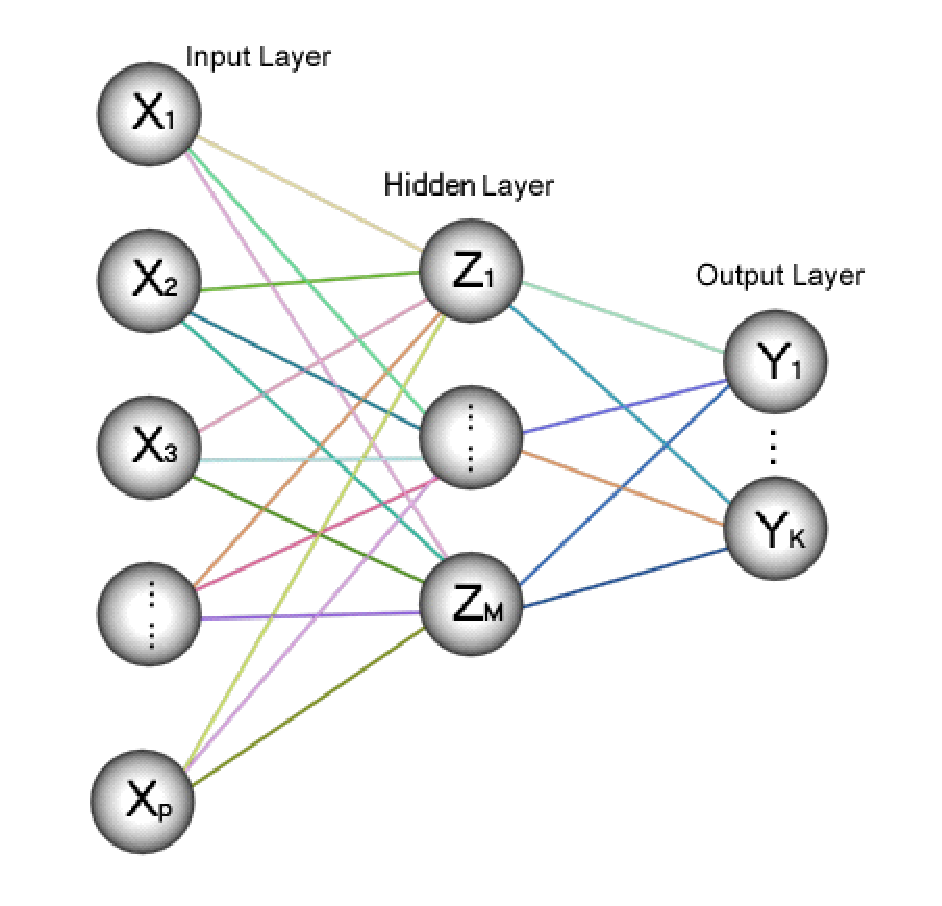
\includegraphics[trim=0 15 0 0,width=0.65\textwidth]{neural_network3.eps}
\caption{Schematic of a single hidden layer, feed-forward neural network.}\label{neural}
\end{figure}

NNs can be modeled with the following formulas:
\begin{eqnarray}
%\begin{aligned}
Z_m &=& \sigma(\alpha_{0m}+\alpha_m^T X)\ , \quad  m =1, \ldots, M \ ,\\
T_k &=& \beta_{0k} + \beta_k^T Z\ , \quad  k = 1, \ldots, K \ ,\\
Y_k &=& f_k(X) = g_k(T) \ , \quad  k =1, \ldots, K\ ,
%\end{aligned}
\end{eqnarray}
where $Z=(Z_1,\ldots,Z_M)$,
$\Theta \equiv \{\alpha_{0m},\alpha_m, m =1, \ldots, M;\beta_{0k}, \beta_k,k =1, \ldots, K\}$
is the set of the model parameters which should be learnt, and $\sigma(v)$ is the \textit{activation function}.

$\sigma(v)$ is usually chosen to be the \textit{sigmoid} function $1/(1+e^{-v})$ or
\textit{Gaussian radial basis} function $\exp\{-\lambda( v-\xi )^2\}$.
Typically $g_k(T)$ is chosen to be the \textit{identity} function $g_k(T)=T$ for regression,
and \textit{softmax} function $g_k(T)=e^{T_k}/ \sum_{l=1}^K e^{T_l}$ for classification.

Sum-of-squared errors are usually used as the measure for regression to fit the NN
\begin{equation}
R(\Theta) = \sum^K_{k=1}\sum^N_{i=1} ( y_{ik}- f_k(x_i))^2 \quad ,
\end{equation}
where $x_i$ and $y_i$ are the $i$-th data point and the real value of the output
in the training data respectively.
For classification, we usually use either squared error or \textit{cross-entropy (deviance)}
as the measure
\begin{equation}
R(\Theta) = -\sum^K_{k=1}\sum^N_{i=1} y_{ik}\log f_k(x_i) \quad ,
\end{equation}
and the corresponding classifier is $G(x)= \arg \max_k f_k(x)$ .

The generic approach to minimizing $R(\Theta)$ is gradient descent, which
is also called \textit{back-propagation} in this setting.
Here we take the sum-of-squared error as an example and show the algorithm detail.
\begin{eqnarray}
\frac{\partial R}{\partial \beta_{km}} &=& -2\sum^N_{i=1}(y_{ik}-f_k(x_i))g'_k(\beta_k^Tz_i)z_{mi} \quad,\\
\frac{\partial R}{\partial \alpha_{ml}} &=& -2\sum^N_{i=1}\sum^K_{k=1}(y_{ik}-f_k(x_i))g'_k(\beta_k^Tz_i)
\beta_{km}\sigma'(\alpha_m^Tx_i)x_{il} \quad,
\end{eqnarray}
where $z_{mi}=\sigma(\alpha_{0m}+\alpha_m^Tx_i)$ and $z_i=(z_{1i},\ldots,z_{Mi})$ .

Given these derivatives, a gradient descent update at the $(t+1)$-th iteration can be done by
\begin{eqnarray}
\beta_{km}^{(t+1)} &=& \beta_{km}^{(t)} - \eta_t \frac{\partial R}{\partial \beta_{km}^{(t)}} \quad , \\
\alpha_{ml}^{(t+1)} &=& \alpha_{ml}^{(t)} - \eta_t \frac{\partial R}{\partial \alpha_{ml}^{(t)}}\quad ,
\end{eqnarray}
where $\eta_t$ is the \textit{learning rate} at the $(t+1)$-th iteration.
Usually $\eta_t$ decreases towards zero when the iteration $t\rightarrow \infty$ \cite{Hastie}.


\subsection{Gaussian Mixture}
Gaussian Mixture models assume that the data points come from $K$ different clusters,
with probability $\pi_k$ in the $k$-th cluster.
The points in the $k$-th cluster are drawn from a Gaussian distribution with mean $\mu_k$
and deviation $\sigma_k$.
Its graphical expression is shown in Figure \ref{gaussian},
where variable $Z_n$ is the class label of the $n$-th data point variable $X_n$ which is a $P$-dimensional vector.
\begin{figure}[h]
\centering
\includegraphics[trim=300 205 220 100,width=0.55\textwidth]{gaussian_mixture2.eps}
\caption{Schematic of a Gaussian Mixture Model.}\label{gaussian}
\end{figure}

We use the maximum log-likelihood estimate
\begin{equation}
R(\Theta) = \sum_{n=1}^N \log P(x_n|\Theta)
= \sum_{n=1}^N \log \big[ \sum_{k=1}^K \pi_k \phi_k(x_n) \big]
\end{equation}
to learn the model parameters
$\Theta=\{\pi_k,\mu_k,\sigma_k; k = 1,\ldots,K\}$,
where $\phi_k(x)$ is the Gaussian density function with mean $\mu_k$ and deviation $\sigma_k$.

The Expectation Maximization (EM) method can be used to solve this problem perfectly
as the label variable $Z$ is considered as the latent variable.
%Typically we can update the parameters iteratively using Expectation Maximization (EM) method.

%For completing this paper, we list the EM algorithm as follows.
%\begin{algorithm}[EM Algorithm]
%\quad
%\begin{enumerate}
%\item \textbf{Expectation Step}:
%\begin{equation}
%Q(\theta, \theta^i) = \int \log (Pr(\theta|X, Z)) Pr(Z|X, \theta^i) dZ \quad ,
%\end{equation}
%where $Z$ stands for hidden variables, $X$ known data and $\theta$ the model parameters.
%\item \textbf{Maximization Step}:
%\begin{equation}
%\theta^{i+1} = \arg \max_\theta Q(\theta, \theta^i) \quad .
%\end{equation}
%\end{enumerate}
%These two steps iterate until $\max|\theta^{i+1} - \theta^i| < \epsilon$,
%where $\epsilon$ is a user-defined small positive number.
%\end{algorithm}

At the E-Step, we calculate the posterior probability of the class label $Z_n$
of the $n$-th point
\begin{equation}\label{posterior}
r_{nk} \equiv P(Z_n=k|x_n,\Theta) = \frac{\pi_k \phi_k(x_n)}{\sum_{l=1}^K\pi_l \phi_l(x_n)} \quad ,
\end{equation}
and at the M-Step, we update the parameters
\begin{eqnarray}
\mu_k &=& \frac{\sum_{n=1}^N r_{nk}x_n}{\sum_{n=1}^N r_{nk}} \quad ,\\
\sigma^2_k &=& \frac{\sum_{n=1}^Nr_{nk}(x_n-\mu_k)^T(x_n-\mu_k)}{P\sum_{n=1}^N r_{nk}} \quad,\\
\pi_k &=& \frac{\sum_{n=1}^N r_{nk}}{N} \quad,\label{pi}
\end{eqnarray}
where $P$ is the dimension of data points.

We update the parameters using equation (\ref{posterior})-(\ref{pi}) until the algorithm converges.

\subsection{Probabilistic Matrix Factorization (PMF)}
\textit{PMF}s \cite{Salak2} are very powerful for Collaborative Filtering problems,
which try to recommend new goods or service to users
according to the historical ratings of the users for goods or service.

PMF supposes the rating value $\pmb R_{u,m}$ of user $u$ for movie $m$ is a normal distribution
with mean $\pmb V_u^T\pmb W_m$ and variance $\eta^2$ given user $u$'s profile $\pmb V_u$ and movie $m$'s
profile $\pmb W_m$. $\pmb V_u$ and $\pmb W_m$ are $K$-dimensional variables.
They have independent normal priors respectively. That is,
\begin{eqnarray}
P(\pmb R_{u,m}|\pmb V_u, \pmb W_m, \eta^2) &=& \mathcal{N}(\pmb R_{u,m}|\pmb V_u^T\pmb W_m, \eta^2) \quad , \\
P(\pmb V_u|\mu, \sigma^2) &=& \mathcal{N}(\pmb V_u|\mu, \sigma^2 \text{I}) \quad, \\
P(\pmb W_m|\theta, \gamma^2) &=& \mathcal{N}(\pmb W_m|\theta, \gamma^2 \text{I}) \quad ,
\end{eqnarray}
where $\Theta\equiv\{\eta^2, \mu, \sigma^2, \theta, \gamma^2\}$ are the model parameters.
PMF also assumes that each of the three distributions is independent for different $u$ and (or) $m$.
Hence the whole probabilistic model can be expressed as follows and its graphical representation is
shown in Figure \ref{graph}.
$\pmb V$ and $\pmb W$ are the \textit{latent variables}.
\begin{align}
P(\pmb R|\pmb V,\pmb W) &= \prod_{(u,m)\in\mathcal{P}} P(\pmb R_{u,m}|\pmb V_u, \pmb W_m, \eta^2)
&=& \prod_{(u,m)\in\mathcal{P}} \mathcal{N}(\pmb R_{u,m}|\pmb V_u^T\pmb W_m, \eta^2) \quad , \\
P(\pmb V|\mu, \sigma^2)\; &= \;\;\;\quad\prod_{u=1}^U P(\pmb V_u|\mu, \sigma^2)
&=& \;\prod_{u=1}^U \mathcal{N}(\pmb V_u|\mu, \sigma^2 \text{I}) \quad, \\
P(\pmb W|\theta, \gamma^2)\; &= \;\;\;\quad\prod_{m=1}^M P(\pmb W_m|\theta, \gamma^2)
&=& \;\prod_{m=1}^M \mathcal{N}(\pmb W_m|\theta, \gamma^2 \text{I}) \quad ,
\end{align}
where $U$ is the number of users and $M$ is the number of goods.
\begin{figure}[h]
    \centering
    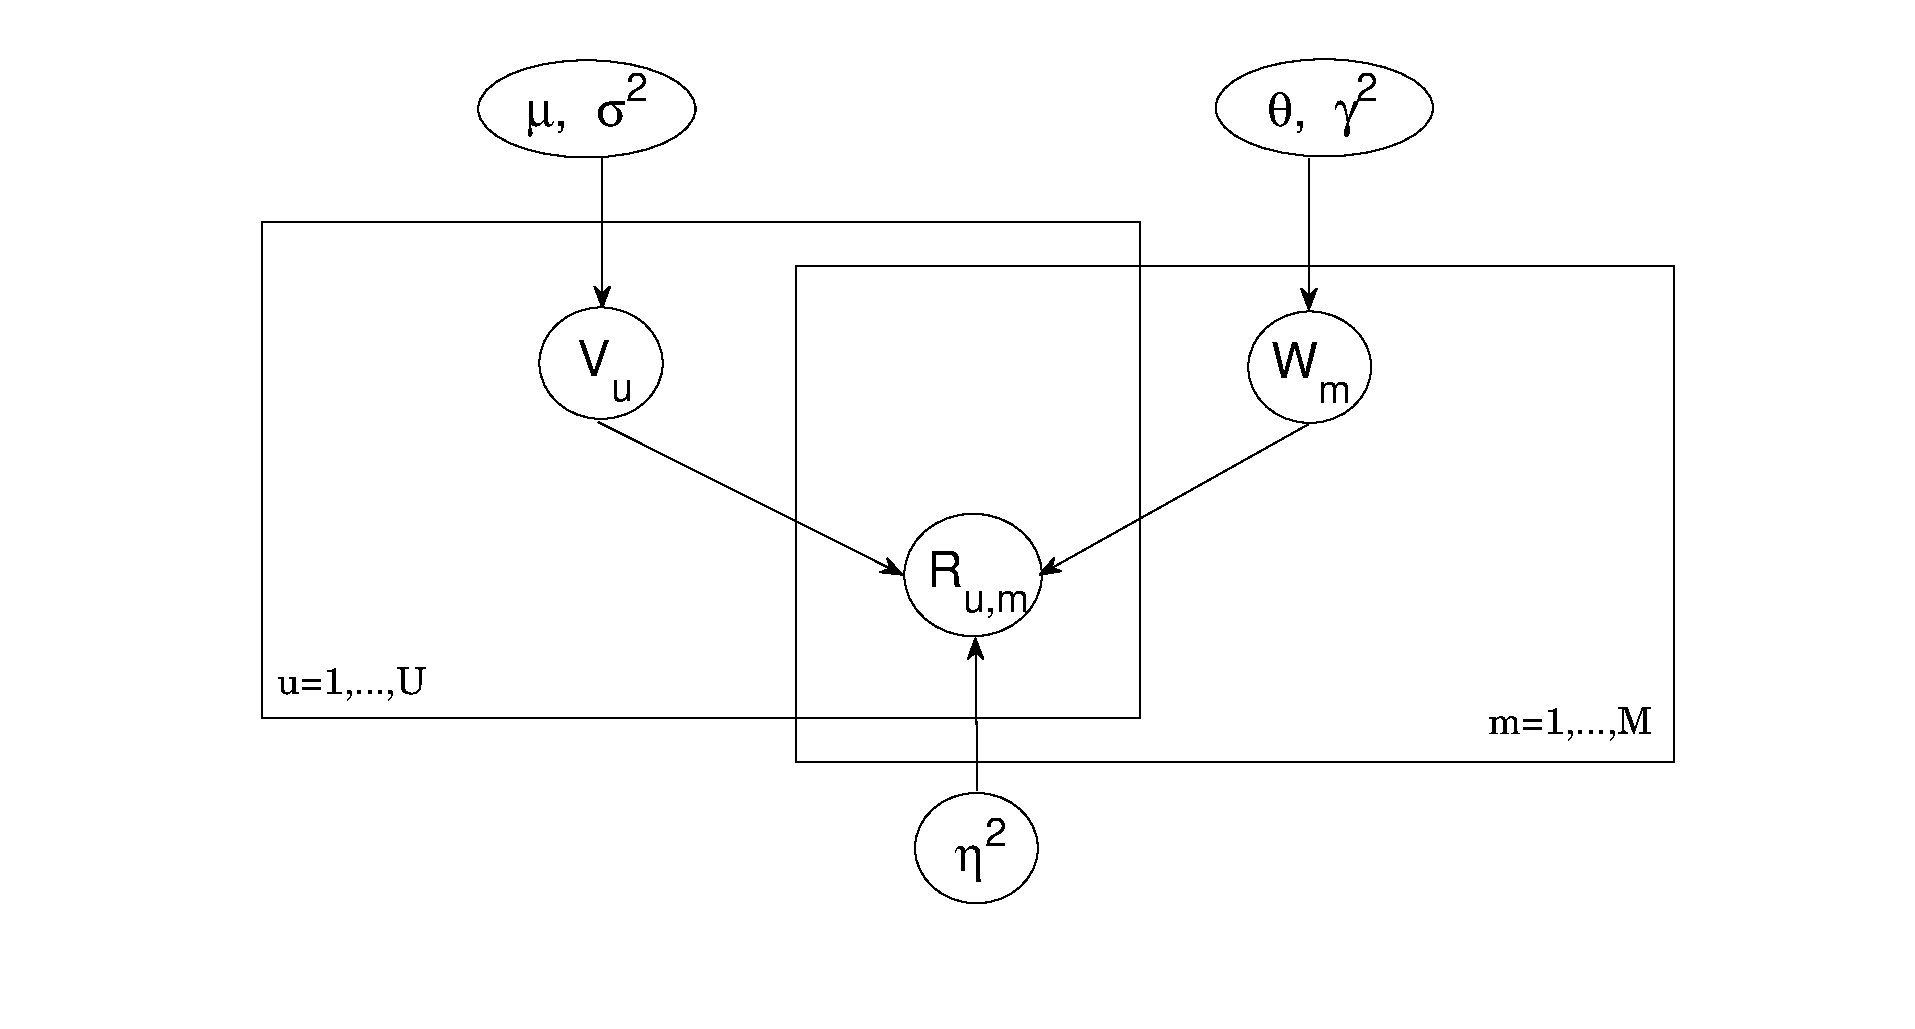
\includegraphics[trim=-10 40 0 0, clip, width=0.80\textwidth]{oriPMF.eps}
    \caption{Schematic of a Probabilistic Matrix Factorization (PMF) model}\label{graph}
\end{figure}

%PMF can be learned using different methods, such as maximum a posteriori (MAP) method,
%variational free energy method and MCMC.
%In the following we use the variational method to solve PMF.

The complete data likelihood is
\begin{equation}\label{likelihood}
\begin{split}
&P(R,V,W|\Theta) = P(R|V,W)P(V|\mu, \sigma^2)P(W|\theta, \gamma^2) \\
&=\prod_{(u,m)\in\mathcal{P}} P(r_{u,m}|V_u, W_m, \eta^2)
\prod_{u=1}^U P(V_u|\mu, \sigma^2)
\prod_{m=1}^M P(W_m|\theta, \gamma^2) \quad .
\end{split}
\end{equation}
The original EM algorithm is not suitable here because
$P(V,W|R,\Theta)$ is computationally difficult since $V$ and $W$ are
not conditionally independent given $R$ and $\Theta$.  The substitution is
the \textit{Variational EM (VEM)}.
VEM assumes that $P(V,W|R,\Theta)$ is approximated by fully factorized $q$-distribution, that is,
\begin{equation}\label{qdist}
    P(V,W|R,\Theta) \simeq Q(V,W) = Q(V)Q(W)
    = \prod_{u=1}^UQ(V_u)\prod_{m=1}^MQ(W_m)  \quad .
\end{equation}

The total variational free energy of PMF with respect to the fully factorized
$q$-distribution is
\begin{equation}
    \begin{aligned}
        &\mathcal{F}(Q(V),Q(W);\Theta) =
        \mathds{E}_{V,W}[\log P(R,V,W|\Theta)-\log Q(V,W)]  \\
        &= -\frac{|\mathcal{P}|}{2}\log (2\pi\eta^2)
        - \mathds{E}_{V,W}\Bigl[\sum_{(u,m)\in\mathcal{P}}\frac{(r_{u,m}-V_u^TW_m)^2}{2\eta^2}\Bigr] \\
        &\quad- \frac{KU}{2}\log(2\pi\sigma^2)
        - \mathds{E}_{V} \Bigl[ \sum_{u=1}^U \frac{(V_u-\mu)^T(V_u-\mu)}{2\sigma^2}\Bigr]\\
        &\quad- \frac{KM}{2} \log(2\pi\gamma^2)
        - \mathds{E}_{W} \Bigl[ \sum_{m=1}^M \frac{(W_m-\theta)^T(W_m-\theta)}{2\gamma^2}\Bigr]\\
        &\quad -\mathds{E}_V\log Q(V) -\mathds{E}_W\log Q(W) \quad ,
    \end{aligned}
\end{equation}
where $K$ is the dimension of $V_u$ and $\mathds{E}_V[f(V)]$ is the expectation of $f(V)$
with respect to the distribution $Q(V)$.
The notation of $\mathds{E}_W[f(W)]$ is defined similarly.

An iterative update procedure can be derived for optimizing the $q$-distribution and the parameters easily.
We will show the detail step by step as follows.

We first work out the update for $Q(V)$.  Differentiating $\mathcal{F}(Q(V),Q(W),\Theta)$
with respect to $Q(V)$ with others fixed, we then set the derivative to $0$
and consider the distribution constraint
$\int Q(V)dV =1$ by Lagrange multipliers method.
\begin{align}
    \frac{\partial \mathcal{F}}{\partial Q(V)}
    &= -\mathds{E}_W\Bigl[\sum_{(u,m)\in\mathcal{P}}\frac{(r_{u,m}-V_u^TW_m)^2}{2\eta^2}\Bigr]
    - \sum_{u=1}^U \frac{(V_u-\mu)^T(V_u-\mu)}{2\sigma^2}
    - \log Q(V) - 1 - \lambda  \notag\\
    &= \quad 0 \notag\\
    \intertext{where $\lambda$ is the Lagrange multiplier.  Hence,}
    Q(V) &\propto \prod_{u=1}^U\exp \left( -\frac12 (V_u-\bar{V}_u)^T\Phi_u^{-1}(V_u-\bar{V}_u) \right )\label{upd_v}\\
    \Phi_u &= \left (\frac{1}{\eta^2}\sum_{m\in\mathcal{P}_u}(\Psi_m+\bar{W}_m\bar{W}_m^T)
    + \frac{1}{\sigma^2} \cdot \text{I} \right )^{-1} \\
    \bar{V}_u &= \Phi_u \left( \frac{1}{\eta^2}\sum_{m\in\mathcal{P}_u}r_{u,m}\bar{W}_m
    + \frac{1}{\sigma^2}\mu \right) \quad .
    \intertext{Similarly we can derive the update step for $Q(W)$,}
    Q(W) &\propto \prod_{m=1}^M\exp \left( -\frac12 (W_m-\bar{W}_m)^T\Psi_m^{-1}(W_m-\bar{W}_m) \right ) \\
    \Psi_m &= \left (\frac{1}{\eta^2}\sum_{u\in\mathcal{P}^m}(\Phi_u+\bar{V}_u\bar{V}_u^T)
    + \frac{1}{\gamma^2} \cdot \text{I} \right )^{-1} \\
    \bar{W}_m &= \Psi_m \left( \frac{1}{\eta^2}\sum_{u\in\mathcal{P}^m}r_{u,m}\bar{V}_u
    + \frac{1}{\gamma^2}\theta \right) \quad .
\end{align}

In the following we derive the update for the parameters.
\begin{align}
    \frac{\partial \mathcal{F}}{\partial \mu}
    &= \frac{\partial}{\partial \mu}\left(
    - \mathds{E}_{V} \Bigl[ \sum_{u=1}^U \frac{(V_u-\mu)^T(V_u-\mu)}{2\sigma^2}\Bigr] \right)\notag \\
    &= \frac{\partial}{\partial \mu}\left(
    - \sum_{u=1}^U \mathds{E}_V\Bigl[
    \frac{[(V_u-\bar{V}_u)+(\bar{V}_u-\mu)]^T[(V_u-\bar{V}_u)+(\bar{V}_u-\mu)]}{2\sigma^2}\Bigr] \right)\notag \\
    &= \frac{\partial}{\partial \mu}\left(
    - \sum_{u=1}^U
    \frac{(\bar{V}_u-\mu)^T(\bar{V}_u-\mu)+\text{trace}(\Phi_u)}{2\sigma^2}\right)\notag \\
    &= \frac{\partial}{\partial \mu}\left(
    - \sum_{u=1}^U\frac{(\bar{V}_u-\mu)^T(\bar{V}_u-\mu)}{2\sigma^2}\right) \notag \\
    &= - \frac{1}{2\sigma^2}\sum_{u=1}^U (2\mu-2\bar{V}_u) \notag \\
    &= 0 \quad . \notag
\end{align}
So,
\begin{align}
    \mu \quad&=\quad \frac{\sum_{u=1}^U\bar{V}_u}{U} \quad .\qquad\qquad\qquad\qquad\qquad\qquad\qquad
    \intertext{Similarly,}
    \theta \quad &= \quad \frac{\sum_{m=1}^M \bar{W}_m}{M} \quad .\qquad\qquad\qquad\qquad\qquad\qquad\qquad
\end{align}

\begin{align}
    \frac{\partial \mathcal{F}}{\partial (\sigma^2)}
    &= - \frac{KU}{2} \frac{1}{\sigma^2}
    - \frac{\partial}{\partial (\sigma^2)}\left(
    \sum_{u=1}^U \mathds{E}_V
    \frac{[(V_u-\bar{V}_u)+(\bar{V}_u-\mu)]^T[(V_u-\bar{V}_u)+(\bar{V}_u-\mu)]}{2\sigma^2} \right)\notag \\
    &= - \frac{KU}{2}\frac{1}{\sigma^2}
    - \frac{\partial}{\partial (\sigma^2)}\left(
    \sum_{u=1}^U
    \frac{(\bar{V}_u-\mu)^T(\bar{V}_u-\mu)+\text{trace}(\Phi_u)}{2\sigma^2}\right)\notag \\
    &= - \frac{KU}{2} \frac{1}{\sigma^2}
    - \frac{\partial}{\partial (\sigma^2)}\left(
    \sum_{u=1}^U
    \frac{(\bar{V}_u-\mu)^T(\bar{V}_u-\mu)+\text{trace}(\Phi_u)}{2\sigma^2} \right)\notag \\
    &= - \frac{KU}{2} \frac{1}{\sigma^2}
    + \frac{1}{2\sigma^4} \sum_{u=1}^U[(\bar{V}_u-\mu)^T(\bar{V}_u-\mu)+\text{trace}(\Phi_u)]\notag\\
    &= 0 \quad . \notag
\end{align}
So,
\begin{align}
    \sigma^2 &= \frac{\sum_{u=1}^U[(\bar{V}_u-\mu)^T(\bar{V}_u-\mu)+\text{trace}(\Phi_u)]}
    {KU} \quad .
    \intertext{Similarly,}
    \gamma^2 &= \frac{\sum_{m=1}^M[(\bar{W}_m-\theta)^T(\bar{W}_m-\theta)+\text{trace}(\Psi_m)]}
    {KM} \quad .
\end{align}

\begin{align}
    \frac{\partial \mathcal{F}}{\partial \eta^2}
    &= -\frac{|\mathcal{P}|}{2\eta^2}
    + \frac{1}{2\eta^4}\mathds{E}_{V,W}\Bigl[\sum_{(u,m)\in\mathcal{P}}(r_{u,m}-V_u^TW_m)^2\Bigr] \notag \\
    &= -\frac{|\mathcal{P}|}{2\eta^2}
    + \frac{1}{2\eta^4}\sum_{(u,m)\in\mathcal{P}}[
    r^2_{u,m}-2r_{u,m}\bar{V}_u^T\bar{W}_m+\text{trace}( (\Phi_u+\bar{V}_u\bar{V}_u^T)(\Psi_m+\bar{W}_m\bar{W}_m^T) )
    ] \notag \\
    &= 0 \quad . \notag
\end{align}
So,
\begin{equation}\label{upd_eta}
    \eta^2 = \frac{1}{|\mathcal{P}|}\sum_{(u,m)\in\mathcal{P}}[
    r^2_{u,m}-2r_{u,m}\bar{V}_u^T\bar{W}_m+\text{trace}( (\Phi_u+\bar{V}_u\bar{V}_u^T)(\Psi_m+\bar{W}_m\bar{W}_m^T) )
    ] \quad .
\end{equation}

We update the $q$-distribution and the parameters iteratively using
Equation \eqref{upd_v}-\eqref{upd_eta} until the algorithm converges.




\begin{thebibliography}{10}

\bibitem{Beal} M. Beal.
\textit{Variational Algorithms for Approximate Bayesian Inference}.
Doctoral thesis, 2003.

\bibitem{Hastie} T. Hastie, R. Tibshirani and J. Friedman.
 The elements of statistical learning.
 \textit{Springer-Verlag}, New York, Berlin and Heidelberg, 2001.

\bibitem{Jordan}
M. I. Jordan, editor.
\textit{Learning in Graphical Models}.
MIT Press, 1999.

\bibitem{Murphy}
Kevin P. Murphy.
\textit{An introduction to graphical models}.

\bibitem{Russell}
S. Russell and P. Norvig.
\textit{Artificial Intelligence: A Modern Approach}.
Prentice Hall, Englewood Cliffs, NJ, 1995.

\bibitem{Salak2} R. Salakhutdinov, and A. Mnih.
Probabilistic Matrix Factorization.
\textit{Advances in Neural Information Processing Systems},
2007.

\end{thebibliography}

%APPENDICES are optional
%\balancecolumns

\end{document}
